\chapter{Problema}\label{chp:problema}

\section{Introdução}\label{sec:problema-introducao}

As organizações, sejam de grandes dimensões ou não, são constituídas por recursos humanos e não-humanos que interagem entre si, através do compartilhamento de recursos físicos ou virtuais, como por exemplo na troca de informações operacionais entre diferentes áreas de uma empresa. Cada uma dessas interações definem processos de negócio que tem por objetivo produzir um resultado para os envolvidos nessa interação extra ou intra-organizacional.

Os processos de negócio, quando realizados de forma desorganizada e despadronizada, levam à ineficiência organizacional pelo simples fato de sua execução não otimizada. Isso ocasiona em elevação dos custos, aumento no retrabalho, insatisfação dos colaboradores e a consequente diminuição na qualidade dos serviços relacionados. Portanto, torna-se altamente necessário uma boa gestão dos processos, a fim de que esses problemas sejam evitados ou mitigados a tempo e não tornem-se um câncer corporativo.

O acesso mais rápido e eficiente às informações estabelece melhores condições para a execução de processos de negócio. Entretanto, não é suficiente para evitar problemas inerentes à presença de informação. A execução despadronizada de processos sem o apoio de um sistema de informação, ou mesmo suportada por sistemas de informação que não acompanham a flexibilidade da constante mudança dos processos, são em geral gargalos fundamentais no insucesso das diversas organizações existentes. A solução desses problemas estabelece melhores condições para a execução, monitoramento e controle de processos, o que termina por aperfeiçoar a tomada de decisão no nível estratégico organizacional.

Neste trabalho, apresentaremos uma alternativa para garantir que a execução das atividades das empresas sejam realizadas da maneira esperada e aumentar a capacidade de monitoramento de cada uma das etapas, que é a automatização de processos. 

\section{Caso de Uso}\label{sec:problema-caso_de_uso}

Ao longo deste trabalho, iremos utilizar o processo descrito a seguir como caso de uso para cada uma das demonstrações de automatização das ferramentas utilizadas para o desenvolvimento da solução proposta.

Em um cenário de operação de um portal de e-commerce, é muito importante a gestão dos preços praticados pela empresa nas diferentes categorias que compõe o mix de produtos ofertados ao consumidor. Erros cometidos por uma precificação manual indevida podem levar a altos prejuízos financeiros e ações na justiça por parte dos consumidores, além de afetar a imagem da corporação perante o mercado. 

O caso ocorrido com a gigante Walmart no portal brasileiro em dezembro de 2013, exemplifica bem o cenário descrito no parágrafo anterior. Neste caso, um computador que custava R\$2.398 reais foi anunciado por R\$580, o que representava um diferença de 75\% a menor em relação ao valor original. Este caso foi noticiado pela imprensa na época, e também houve bastante repercusão nas redes sociais, deixando muitos clientes insatisfeitos pelo cancelamento da compra (http://oglobo.globo.com/economia/defesa-do-consumidor/walmart-erra-preco-de-produto-em-site-cancela-venda-irrita-clientes-11098550). 

Nesse sentido, torna-se necessário a implantação de um processo de precificação manual que envolva a avaliação de regras que limitem a troca de preço sem a aprovação de alçadas superiores. Essa nova gestão tem por objetivo trazer mais qualidade e segurança nas mudanças de preço solicitadas pelos diferentes precificadores das categorias do site, alinhando assim a gestão de preços do portal e evitando trocas de preço equivocadas ou não autorizadas pelos gestores.

O processo inicia com a decisão do analista de uma determinada categoria de produtos do site, pela mudança de preço de um SKU. O novo preço do SKU é definido pelo analista e enviado para aprovação.

A solicitação enviada pelo analista é avaliada quanto a regra de alçada definida pelos gestores, e caso possua uma variação de preço acima de 30\%, deve passar pela aprovação de dois gestores. Em um cenário real de negócios, certamente a regra seria mais complexa, como por exemplo variando em função da categoria do produto. Entretanto, assumiremos a regra da variação de 30\% nas demonstrações como forma de simplificar o entendimento e aplicação das regras de negócio estabelecidas para o processo.

Após a avaliação da variação de preço, caso tenha sido acima de 30\%, o processo deve ser encaminhado para a aprovação de dois gestores. Caso a variação seja menor ou igual a 30\%, a mudança não requer aprovação. Após isso, a troca de preço será efetuada no portal.

A imagem a seguir descreve de forma visual o fluxo do processo descrito anteriormente:

\begin{figure}[H]
  \centering
  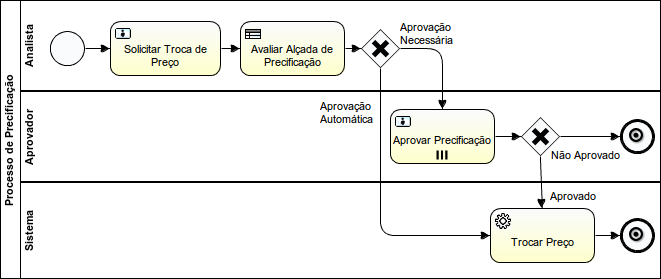
\includegraphics[width=1.0\textwidth]{imagens/ProcessoDePrecificacao.png}
  \caption{Processo de Precificação Manual}
  \label{fig:exemplo_bpmn}
\end{figure}